\documentclass{article}
\usepackage{graphicx}
\usepackage[strings]{underscore}
\usepackage{url}
\usepackage[margin=2cm]{geometry}

\usepackage{titlesec}


\title{Large Dynamic Voxel Scenes using Sparse Voxel Octrees}
\author{Nicolas Fedor, 6683787}
\date{May 2025}

\begin{document}
\maketitle

\section{Introduction}
Voxel rendering has become an essential technique in computer graphics, enabling the representation and visualization of 3D environments through volumetric data. Unlike traditional polygon-based methods that rely on triangles and surface meshes, voxel rendering represents scenes as a grid of volumetric elements (voxels), which allows for detailed depictions of complex structures such as terrains, clouds, or medical imaging data. This approach offers several advantages, particularly in handling volumetric and procedural data, but also poses significant challenges, including high memory consumption and computational demands.

Several data compression techniques have been developed to address these challenges, such as Sparse Voxel Octrees (SVOs) and Sparse Voxel Directed Acyclic Graphs (SVDAGs). These methods aim to reduce memory usage by representing voxel data in a hierarchical, sparse format, allowing for efficient storage and rendering of large voxel grids. However, dynamic scenes present additional challenges, as updating the highly compressed voxel data structure in real-time can be computationally expensive.

This project will explore the usage of an SVO for rendering a large world and the challenges of dynamic voxel data. By optimizing the construction of the SVO, and creating a clear separation of static and dynamic voxel data, this work aims to achieve real-time rendering of dynamic voxel worlds.

\subsection{Aims and Objectives}
The aim of this project is to develop a dynamic voxel rendering system using an SVO data structure. There are two main objectives:

\begin{itemize}
    \item Design and implement an SVO data structure for representing voxel data.
    \item Optimize SVO updates for real-time rendering of dynamic voxel worlds.
\end{itemize}

\subsubsection{Sparse Voxel Octree Data Structure}
Voxel data can take up a large amount of memory, especially for high-resolution grids. The SVO data structure aims to compress the voxel data by representing the volume as a tree of nodes, where each node contains either a single voxel or a pointer to a child node. This hierarchical representation allows for efficient storage and traversal of the voxel data, reducing the memory footprint and improving rendering performance. The objective is to design and implement an SVO data structure that can efficiently store and render large voxel worlds, using previous works as a reference~\cite{Laine_Karras_2010}.

\begin{itemize}
    \item Design and implement an SVO data structure for representing voxel data.
    \item Optimize SVO construction and traversal for real-time rendering.
    \item Achieve a minimal memory footprint for rendering large voxel worlds.
\end{itemize}

Many different techniques have been developed to optimize the construction and traversal of SVOs, such as using Morton codes to encode the voxel data and improve cache coherency~\cite{Laine_Karras_2010}. The aim isn't to identify new compression methods but to implement these existing techniques and evaluate their performance in the context of dynamic voxel rendering. Using the work of Laine and Karras as a reference, the target is to, using a 1024\textsuperscript{3} voxel grid:

\begin{itemize}
    \item Aim for a memory footprint of 1GB or less.
    \item Cast 20 million rays per second, at a resolution of 1920x1080.
    \item Achieve a frame rate of 30fps or higher.
\end{itemize}

\subsubsection{Dynamic Voxel Data}
Dynamic voxel data presents additional challenges, as updating the voxel grid in real-time can be computationally expensive. The objective is to optimize the SVO updates for dynamic voxel worlds, by separating static and dynamic voxel data, and efficiently updating the SVO structure to reflect changes in the voxel grid. This will involve developing techniques for efficiently updating the SVO while maintaining real-time rendering performance, based on previous works~\cite{Crassin_2012}. Using the same 1024\textsuperscript{3} voxel grid:

\begin{itemize}
    \item Achieve a frame rate of 30fps or higher with dynamic voxel updates.
    \item Merging of static and dynamic voxel data should be done in real-time, without affecting frame rate.
\end{itemize}

\section{Literature Review}
This chapter will provide an overview of the existing techniques for rendering voxel data, including traditional mesh-based methods and recent advances using ray tracing and sparse voxel representations.

\subsection{Mesh-based Rendering}
Mesh-based rendering is the most common technique for representing 3D objects in computer graphics. It involves defining the surface of an object using a collection of polygons, typically triangles, which are then rendered using the GPU's rasterization pipeline. This is a well-established approach, that is the default method for rendering 3D graphics in most applications.

Volumetric voxel data can be converted to a mesh representation using techniques such as Marching Cubes~\cite{Amran_1998}, which extract the surface of the volume by sampling the voxel data; or another simpler, popular, approach is to use greedy meshing~\cite{mikolalysenko_2012}, which relies on creating a mesh by merging adjacent voxels with the same material into a single quad face in the mesh, see Figure~\ref{fig:greedy}. These approaches allow for storing voxel data uncompressed and so dynamic updates to voxel data are quick. However, the generation of the mesh becomes a bottleneck as the resolution of the voxel data increases.

\begin{figure}[thp]
    \begin{center}
        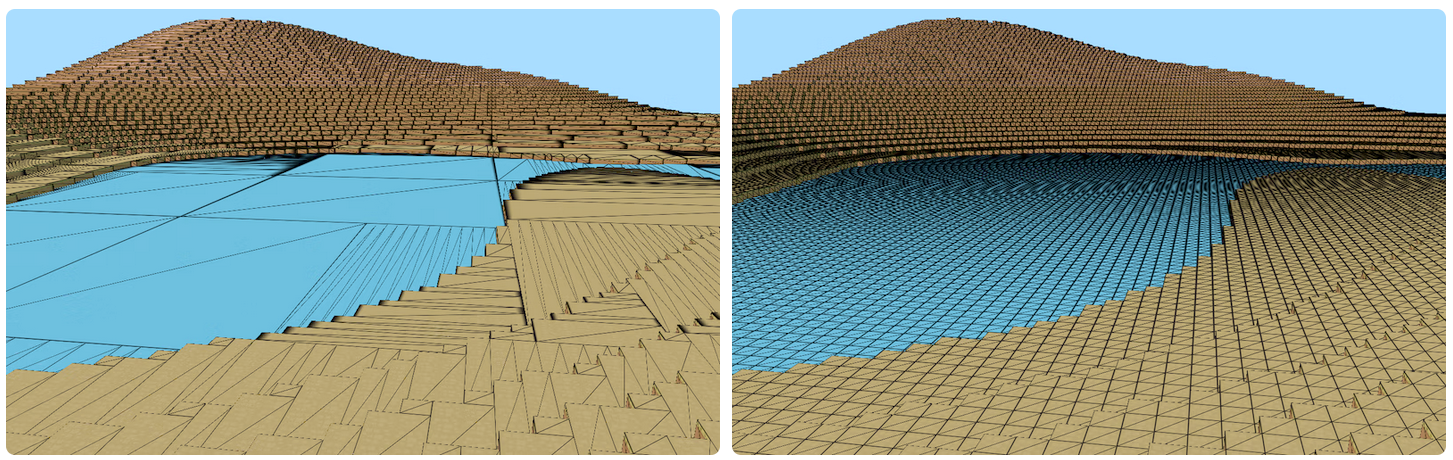
\includegraphics[width=0.8\textwidth]{figures/greedy.png}
    \end{center}
    \caption{Comparison of creating a mesh for voxel data with (left) and without (right) greedy meshing~\cite{Gedge_2014}.}
    \label{fig:greedy}
\end{figure}

\subsection{Ray Marching}
Ray marching, a specialized form of ray tracing, is another technique for rendering voxel data. It involves casting a ray through a 3D grid of voxels and sampling the voxel data along the ray to determine the color and opacity of the volume at each point. Ray marching can be implemented on the GPU using compute shaders, avoiding the creation of a mesh, instead the GPU can operate directly on the voxel data, which can be stored in a compressed format.

\subsubsection{Digital Differential Analysis (DDA)}
A common technique for ray marching is Digital Differential Analysis (DDA), which involves stepping through the voxel grid along the ray using fixed-size increments or steps calculated based on the ray direction, see Figure~\ref{fig:dda}. At each step, the voxel data is sampled to determine the color and opacity of the volume, which is accumulated along the ray to produce the final image. DDA is a simple and efficient method for ray marching~\cite{Amanatides_Woo_1987}, but intersection testing a ray is an expensive operation and so limiting the number of intersection tests a ray tracer must perform is important for real-time rendering.

\begin{figure}[thp]
    \begin{center}
        \scalebox{0.5}{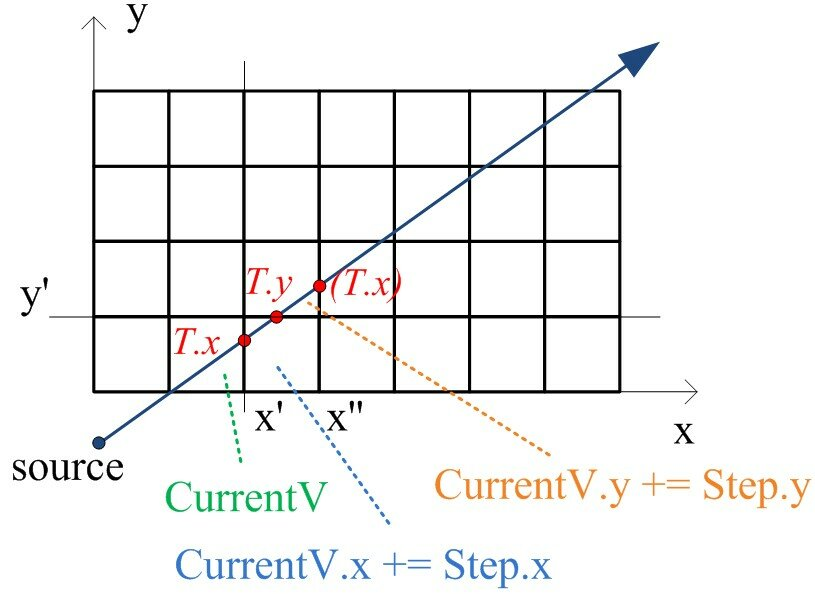
\includegraphics[width=0.8\textwidth]{figures/dda.jpg}}
    \end{center}
    \caption{Illustration of the steps in Digital Differential Analysis (DDA) for ray marching~\cite{Xiao_2019}.}
    \label{fig:dda}
\end{figure}

\subsection{Data Compression}
Compressing a voxel grid is essential for rendering large voxel worlds efficiently using ray marching as the number of intersection tests has a large impact on ray tracing performance, in ray tracing Binary Space Partitioning is a way of improving ray tracing performance~\cite{Ize_2009}.

Sparse Voxel Octrees (SVOs) emerged as a popular solution to compressing voxel data. SVOs are a hierarchical data structure that represents a voxel grid as a tree of nodes, where each node contains either a single voxel or a pointer to a child node; the aim here is to reduce the memory usage by storing only the voxels that are necessary to represent the volume i.e. by collapsing "chunks" of similar voxels into a single node. An example of an SVO is shown in Figure~\ref{fig:svo}.

\begin{figure}[thp]
    \begin{center}
        \scalebox{0.5}{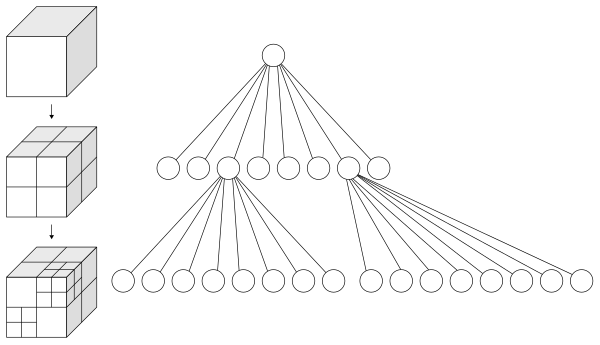
\includegraphics[width=0.8\textwidth]{figures/octree.png}}
    \end{center}
    \caption{Illustration of an Octree representation of a voxel grid. Source: Wikipedia}
    \label{fig:svo}
\end{figure}

Additional techniques for compression voxel data like Sparse Voxel Directed Acyclic Graphs (SVDAGs) have been proposed and these are even better suited to storing large, high-resolution voxel worlds~\cite{Kampe_Sintorn_Assarsson}.

\subsection{Dynamic Voxel Data}
Minecraft is a voxel-based video game that makes use of mesh-based rendering~\label{Mesh-based Rendering} to render its voxel world. The game supports dymanic updates to the voxel world by separating the world into smaller chunks, which can be updated independently of each other. This allows for efficient updates to the voxel data, as only the affected chunks need to be modified, and the rest of the world can remain static.

Another approach for voxel modification is by storing an "overlay" of the modified voxels on top of the static voxel data. In ray marching, initial rays are cast through the static voxel data, and then the overlay can be checked for any modifications to the voxel data. This approach allows for dynamic updates to the voxel world without modifying the underlying voxel data. Since SVOs are hierachical in their nature, it is possible to store the overlay as a separate SVO, which can be merged with the static SVO~\cite{Douglas_2022} at a later stage.

\section{Technical Overview}
This chapter will provide a technical overview of the proposed dynamic voxel rendering system.

\subsection{Voxel Data Representation}
The voxel world will consist of two SVO data structures; a static SVO that cannot be modified directly and is used for rendering the voxel world, and a dynamic SVO that stores the modified voxel data. The dynamic SVO will be used to store the overlay of the modified voxels, which can be merged with the static SVO to update the voxel world.

There will be a single voxel attribute, color, that will be stored uncompressed in the SVO nodes. The color will be represented as a 32-bit RGBA value, which can be used to determine the color and opacity of the volume at each point. The SVO will be stored uncompressed in memory on the CPU, but will be compressed to a 1D array of nodes using morton code for efficient storage and traversal on the GPU, see Figure~\ref{fig:svo_to_morton}.

\begin{figure}[thp]
    \begin{center}
        \scalebox{0.5}{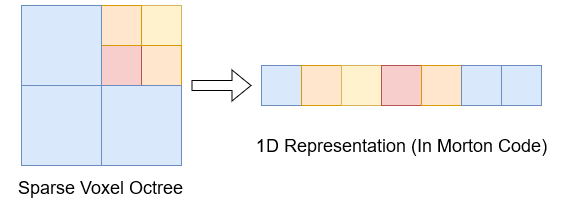
\includegraphics[width=0.8\textwidth]{figures/svo_to_morton.png}}
    \end{center}
    \caption{Conversion of an SVO to a 1D array of nodes using Morton code, illustrated as a quadtree for simplicity.}
    \label{fig:svo_to_morton}
\end{figure}

The morton, or Z-ordering, is calculated by interleaving the X, Y, and Z coordinates of the voxel data to create a single index that preserves locality in 3D space, see Figure~\ref{fig:morton}.

\begin{figure}[thp]
    \begin{center}
        \scalebox{0.5}{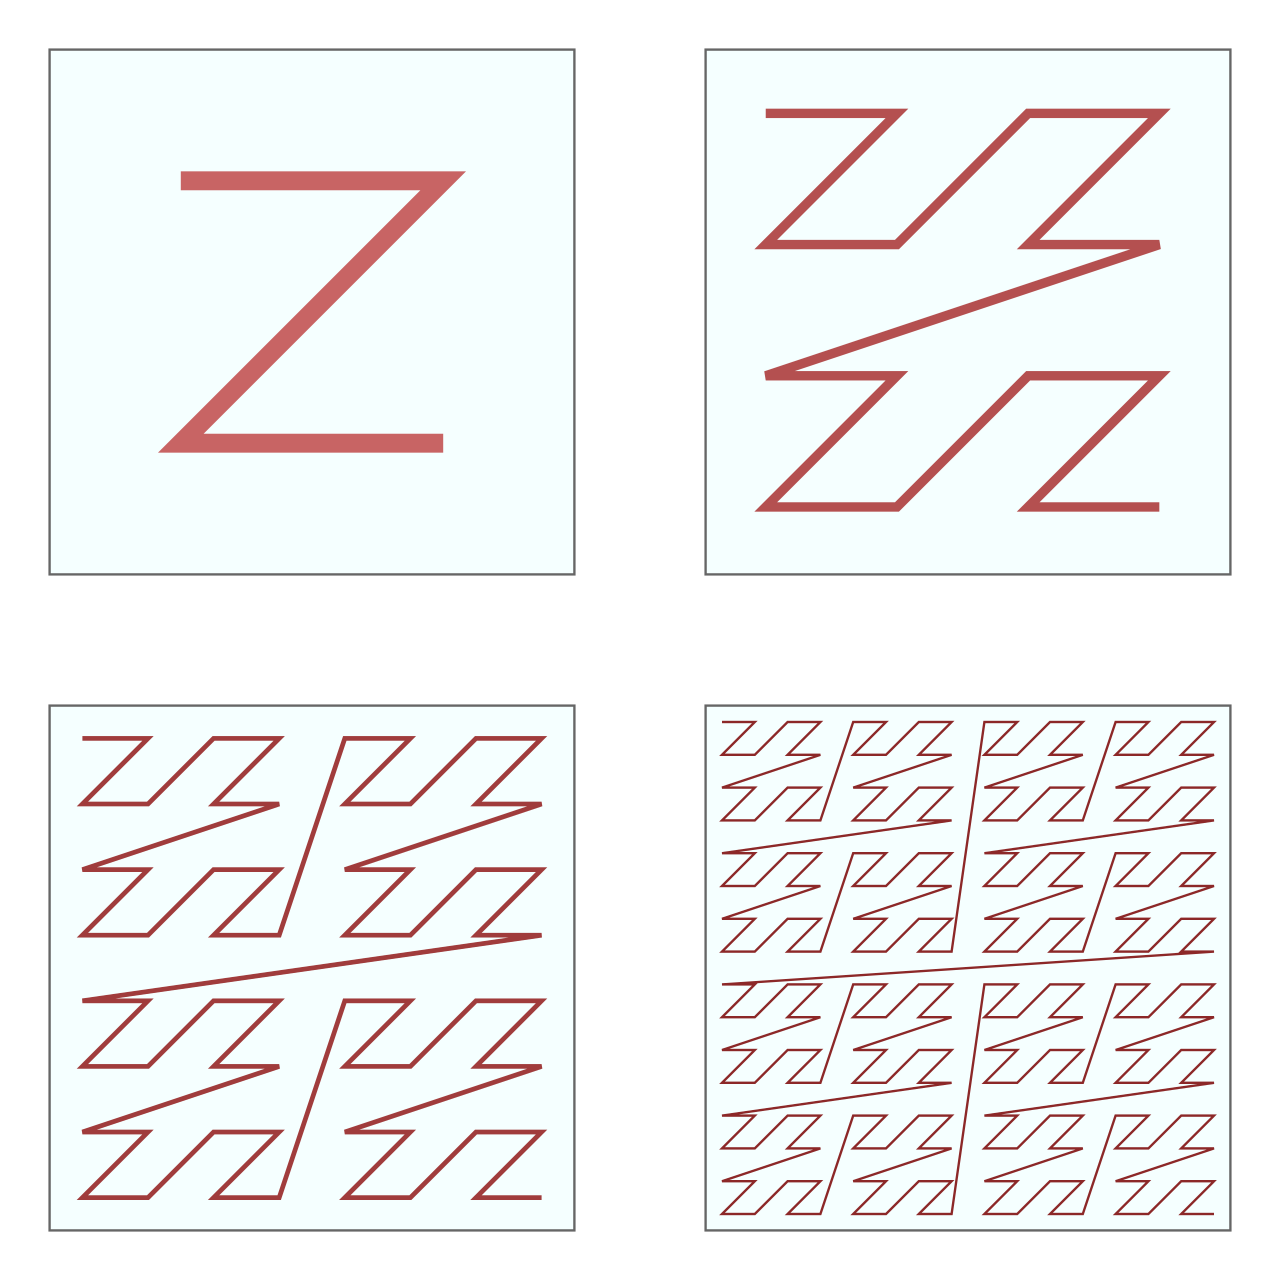
\includegraphics[width=0.8\textwidth]{figures/morton.png}}
    \end{center}
    \caption{Voxels are traversed in a 'Z' pattern to create a Morton code, illustrated using a 2D grid for simplicity. Source: Wikipedia}
    \label{fig:morton}
\end{figure}

\subsection{Graphical Pipeline}
While the exact rendering techniques are not the focus of this project, a brief overview of the graphical pipeline is provided for context. The voxel data will be rendered using ray marching, which involves casting a ray through the voxel grid and sampling the voxel data along the ray to determine the color and opacity of the volume at each point. The ray marching algorithm will be implemented on the GPU using compute shaders, which can operate directly on the voxel data stored in the SVO; Vulkan 1.3 will be used as the graphics API as it allows granular control over memory on the GPU which will be important for optimizing the updating of the SVO. See Figure~\ref{fig:graphical_pipeline} for an overview of the proposed graphical pipeline.

\begin{figure}[thp]
    \begin{center}
        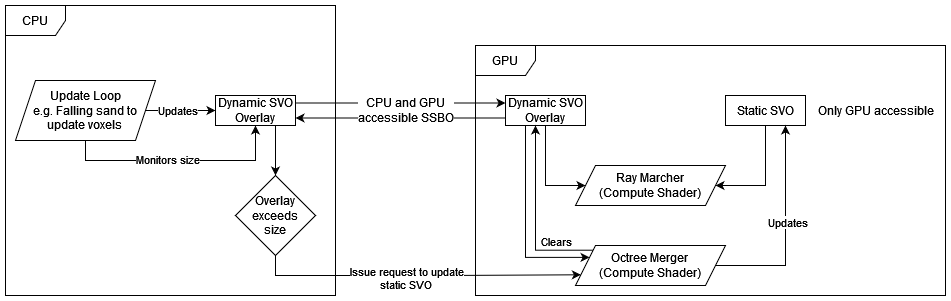
\includegraphics[width=0.8\textwidth]{figures/graphical_pipeline.png}
    \end{center}
    \caption{Overview of how the CPU and GPU interact to render the voxel world, and apply dynamic updates.}
    \label{fig:graphical_pipeline}
\end{figure}

\subsection{Dynamic Voxel Updates}
The dynamic SVO will store the overlay of the modified voxels, which can be merged with the static SVO to update the voxel world. The dynamic SVO will be updated in real-time as the voxel data is modified, and the changes will be applied to the static SVO at a later stage. The dynamic SVO will be stored in GPU memory in the same compressed format as the static SVO.

The ray marcher will trace through the static SVO first, and then check the dynamic SVO for any modifications to the voxel data. The dynamic SVO will be merged with the static SVO at the end of each frame, and the changes will be applied to the voxel world. The merging process will involve updating the static SVO with the modified voxels from the dynamic SVO, and then compressing the SVO back to a 1D array of nodes using morton code.

\section{Workplan}
This section will highlight the key milestones and timeline for the project. Given the complexity of the project, there are also several risks that could impact the success of the project.

\subsection{Timeline}
The project will be divided into several phases, each focusing on a specific aspect of the dynamic voxel rendering system. The timeline for the project is as follows:

\begin{itemize}
    \item \textbf{Phase 1 (Weeks 1-4):} Research and design of the SVO data structure.
    \item \textbf{Phase 2 (Weeks 5-8):} Implementation of the SVO data structure and optimization of the construction and traversal algorithms.
    \item \textbf{Phase 3 (Weeks 9-12):} Research and design of the dynamic voxel updates.
    \item \textbf{Phase 4 (Weeks 13-16):} Implementation of the dynamic voxel updates and optimization of the merging process.
    \item \textbf{Phase 5 (Weeks 17-20):} Integration of the SVO data structure and dynamic voxel updates into the graphical pipeline.
    \item \textbf{Phase 6 (Weeks 21-24):} Evaluation of the system and optimization of the performance.
\end{itemize}

\subsection{Risks}
Voxel rendering can become a very challenging area to work in as there are many different techniques and systems that can be used and built upon. Creating a voxel rendering system that can render large voxel worlds in real-time is a challenging task, and there are several risks that could impact the success of the project:

\begin{itemize}
    \item Inadequate performance: The ray marching algorithm may not be able to render the voxel world in real-time, or the SVO may not be able to store and render large voxel worlds efficiently.
    \item Vulkan Requirement: Vulkan is a low-level graphics API that requires a good understanding of the GPU architecture and memory management, which could be a barrier to implementing the graphical pipeline.
    \item Dynamic Updates: The dynamic SVO may not be able to store and update the modified voxel data in real-time, or the merging process may not be able to apply the changes to the static SVO efficiently resulting in suboptimal performance.
    \item Interaction between CPU and GPU: The interaction between the CPU and GPU is typically a bottleneck and transferring a large amount of data between the two needs consideration. The SVO will be stored in CPU memory and then transferred to GPU memory for rendering, which could hinder rendering times as the SVO grows in size.
    \item Octree Merging: Merging the dynamic SVO and static SVO will be done on the GPU. Frame synchronization should be made use of to only merge the octrees when the GPU isn't otherwise actively rendering as this would have a negative impact on frame rate.
\end{itemize}

Performance and memory footprint are a key success metric for this project, and the risks outlined above could impact the ability to achieve the project objectives.

\bibliographystyle{IEEEtran}
\bibliography{references}

\end{document}
